\newpage
\section{Architecture}
\subsection{Server}
The back-end server is divided into two parts with an underlying database connection. 
The first part is responsible for fetching data from the user's home from the Home Data Aggregator and store
this data in the database for future use. The second part is responsible for communicating with the application on the 
Android device. It will fetch data about a user's specific usage, the user's friends usage, or general statistics 
concerning power usage. The database connection layer will serve as an abstraction to the database itself and provide 
easy access to the data stored.

\begin{figure}[H]
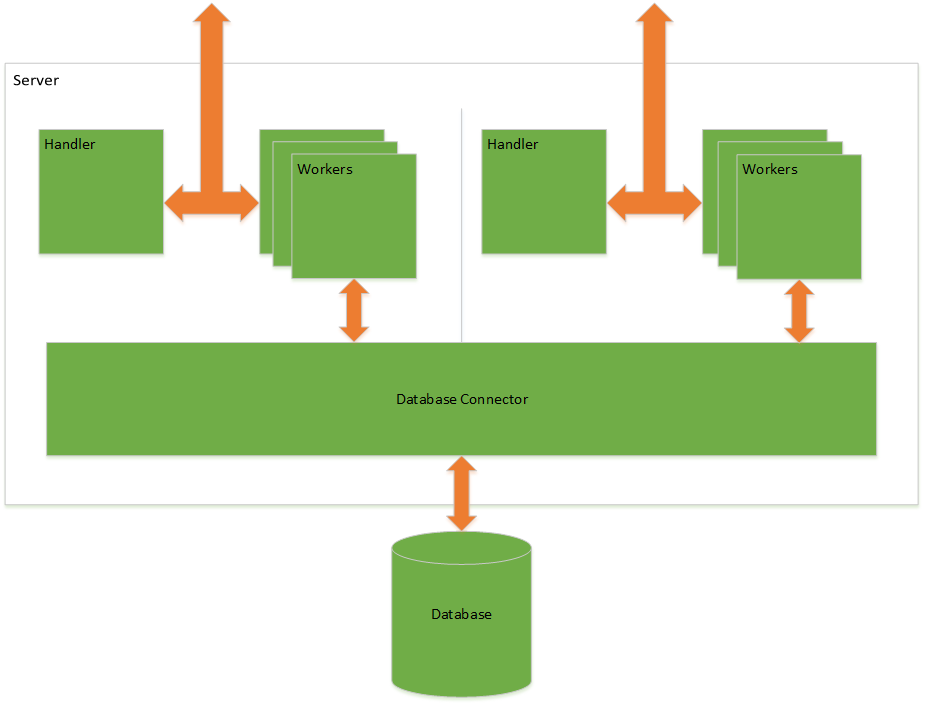
\includegraphics[width=\textwidth]{ch/projectPlan/fig/server.png}
\caption{Server}
\end{figure}

\subsection{Android Device}
The application running on the Android device will be responsible for handling connections to external 
services like the APIs of Google Drive and Facebook and combine them with data from the server in order to represent 
data to the user.

\begin{figure}[H]
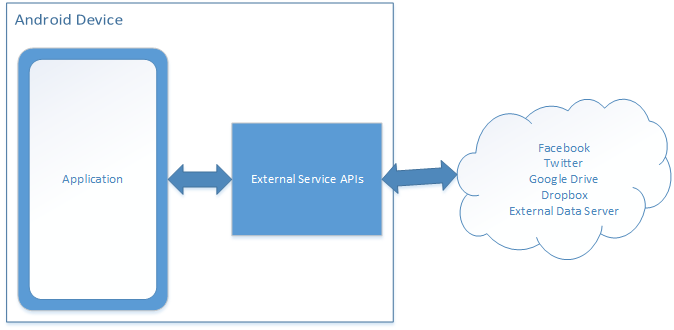
\includegraphics[width=\textwidth]{ch/projectPlan/fig/androidDevice.png}
\caption{Android device}
\end{figure}

\subsection{Home Data Aggregator}
This device will collect data from sources in the user's home. The reason for this external box as opposed to using 
the user's phone to collect data, is that with this solution the system can fetch data at regular intervals throughout 
the whole day. This would result in that the user would not need to be home in order for the application to collect 
usage data. The device will pass data along to the external server at request from the server.

\begin{figure}[H]
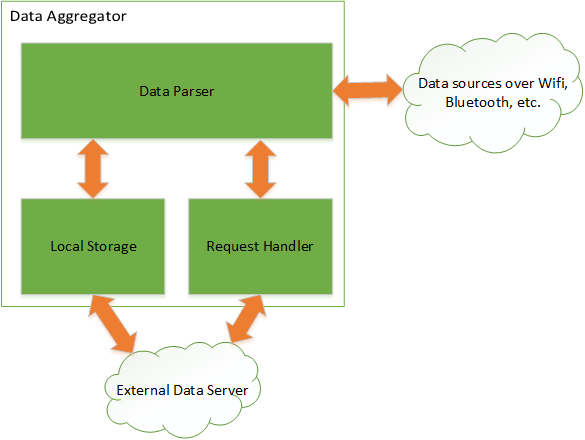
\includegraphics[width=\textwidth]{ch/projectPlan/fig/home.png}
\caption{Home data aggregator}
\end{figure}
